\documentclass{article}

\usepackage{ctex}
\usepackage{lastpage}
\usepackage{pdflscape}
\usepackage{longtable}
\usepackage{tabu}
\usepackage[bottom=3.5cm,left=1.5cm, right=1.5cm]{geometry}
\usepackage{fancyhdr}
\pagestyle{fancy}

\newcommand{\reporttitle}{染色体异常检测(WGS-CAT)临床报告单}
\newcommand{\reportuniqueid}{LE201709091001}

\newcommand{\drawhline}{\noindent \centerline{\rule{\textwidth}{2pt}}}

\newcommand{\headingone}[1]{{\noindent \Large \kaishu{#1}}\\}

\lhead{\setlength{\unitlength}{1em}
	\begin{picture}(0,0)
	\put(0,0){
\includegraphics[width=6em]{./figures/logo.pdf}}
	\end{picture}}

\chead{\textbf{北京乐土医学检验所}} 
\rhead{\textbf{\reportuniqueid}} 
\cfoot{第\thepage 页/共\pageref{LastPage} 页 \\
	地址:北京市中关村生命科学园北大医疗产业园15号3层\\
	邮箱:CL-HEALTH@cheerlandgroup.com\\
	网址:www.cheerlandgroup.com\\
	电话:4001-566-966
}

\renewcommand{\headrulewidth}{0.4pt}

\renewcommand{\footrulewidth}{0.4pt}

\title{\reporttitle}
\date{}

\begin{document}
	\centerline{\huge \reporttitle}
	
	\drawhline
	\section*{基本信息}
	
\begin{table}[h]
	\centering
	\begin{tabular}{cll||cll||cll}
		\hline
		送检单位 & : & 京州市第一人民医院 & 送检部门 & : & 妇产科       & 门诊号  & : & JZ20171021  \\
		姓\qquad 名   & : & 贾德仁 & 性\qquad 别   & : & 男 & 出生日期 & : & 1985年10月27日 \\
		样本编号 & : & \reportuniqueid & 样本类型 & : & 血液 & 采样方式 & : & 左臂静脉采血      \\
		采样时间 & : & 2017年8月2日      & 收样日期 & : & 2017年8月4日 & 寄送方式 & : & 冷链速运        \\
		\hline
		临床描述 & : & \multicolumn{7}{l}{\begin{minipage}{0.8\textwidth}
				结婚五年,未能成功怀孕。
		\end{minipage}}                                        
	\end{tabular}
\end{table}

\drawhline
\section*{检测方法}
% \headingone{检测方法}


\noindent \begin{tabular}{ccl}
	检测项目 & : & 染色体异常检测 \\
	检测方法& : & 全基因组高通量测序分析\\
\end{tabular} 

\section*{检测结果}
%\headingone{检测结果:}

\begin{longtabu} to \textwidth {|c|l|c|c|}
	\hline
	\textbf{检测项目} & \multicolumn{1}{c|}{\textbf{染色体异常}}  & \textbf{异常类型} &  \textbf{备注}\\ \hline
	\endhead
		染色体数目异常 & 无 & 无 & 无\\ \hline
	染色体结构异常 & chr19\_14231120\_24231120\_chr1\_134231120\_194231120;  & 易位 & 平衡易位\\ \hline
	染色体结构异常 & chr2\_0\_84231120\_chr10\_74231120\_114231120;  & 易位 & 平衡易位\\ \hline
	染色体结构异常 & chr12\_94231120\_124231120\_chr18\_24231120\_74231120; & 易位 & 平衡易位\\ \hline
	染色体结构异常 & chrX\_94231120\_124231120\_chrY\_4231120\_9231120; & 易位 & 平衡易位\\ \hline
	染色体结构异常 & chr1:23230983-43330983; & 缺失 & \\ \hline
	染色体结构异常 & chr5:34231120-44231120; & 缺失 & \\ \hline
	染色体结构异常 & chrY:34231120-44231120; & 缺失 & \\ \hline
	染色体结构异常 & chr11:123230983-123330983; & 重复 &\\ \hline
	染色体结构异常 & chr7:74231120-84231120; & 重复 & \\ \hline
	染色体结构异常 & chr11:120530983-120630983; & 重复 & \\ \hline
	染色体结构异常 & chr18:4231520-14222120; & 重复 & \\ \hline
	染色体结构异常 & chrX:4231520-14222120; & 重复 & \\ \hline
	染色体结构异常 & chr3:74231120-84231120; & 倒位 &\\ \hline
	染色体结构异常 & chr13\_78231120\_78291120\_chr16\_74231120\_84231120;  & 易位插入 &\\ \hline
\end{longtabu}

\section*{结果说明}
%\headingone{结果说明:}

多篇文献报道,第 18 号染色体 q22 区域周围存在与生殖相关的基因,该断裂处发生的平衡易位可能会导致反复流产、男性生殖器官发育不全等[1-2]。 

…… 

chr11\_120530983\_120630983 区段为 11 号染色体的一段 100Kb 区域的杂合缺失,为临床意义未明变异。该区域内有 HMGCS1; IL7R;等 2 个基因,历史上没有相关基因的致病性案例报道;2 个基因中,暂无在 OMIM 收录的疾病相关基因。
 
…… 

\section*{遗传咨询}

%\headingone{遗传咨询:}

根据孟德尔第一平衡定律,染色体平衡易位携带者婚配后生育染色体异常后代的危险率高达 50$\sim$100\%。配偶中一方为某一常染色体平衡易位携带者,另一方正常,根据配子形成中同源染色体节段相互配对的特性,经过分离与交换,理论上形成 18 种类型的配子,它们分别与正常的配子结合,则可形成 18 种类型的合子,其中仅有一种正常,一种为表型正常的平衡易位携带者,其余 16 种均不正常。该受检者下次再妊娠需进行产前诊断及遗传咨询。

\section*{参考文献}
%\headingone{参考文献:}

1.Stephenson MD,Sierra S.Reproductive outcomes in recurrent pregnancy loss associated with a parental carrier of a structural chromosome rearrangement.Hum Reprod,2006,21(4):1076—1082.
 
2.ESHRE Capri Workshop Group.Genetic aspects of female reproduction.Hum Reprod Update,2008,14(4):293—307.

\section*{建议与解释}
%\headingone{建议与解释:}

\begin{enumerate}
	\item 本检测结果仅对送检的该样本负责。 
	\item 该方法不适宜检测:样本接受过异体输血、移植手术、干细胞治疗、免疫治疗等。
	\item 该检测,鉴于当前医学检测技术水平的限制和个体差异等不同原因,即使在检测人员已经履行了工作职责和操作规程的前提下,仍有可能出现假阳性或假阴性。
	\item 本检测结果仅供参考,不作为最终诊断结果,相关解释请咨询临床医生。
	\item 受检者和送检方需提供完整、准确、详实的个人资料。因受检者提供的用户资料不实或其它误导因素而导致检测服务的中断、结果不准确,本中心对此不承担责任。
	\item 本中心对该结果保密并依法保护用户的隐私,但因受检者个人原因出现的信息外泄,本中心不承担相应责任。
	\item 本检测鉴于当前医学检测技术水平的限制和个体差异等不同原因,只报告超过 100Kbp 大小的 DNA 片段的结构变异。
	\item 本检测报告所报道的异常位置是基于 GRCh37/hg19 的参考序列。
\end{enumerate}

\newpage

\begin{landscape}
	\begin{figure}
		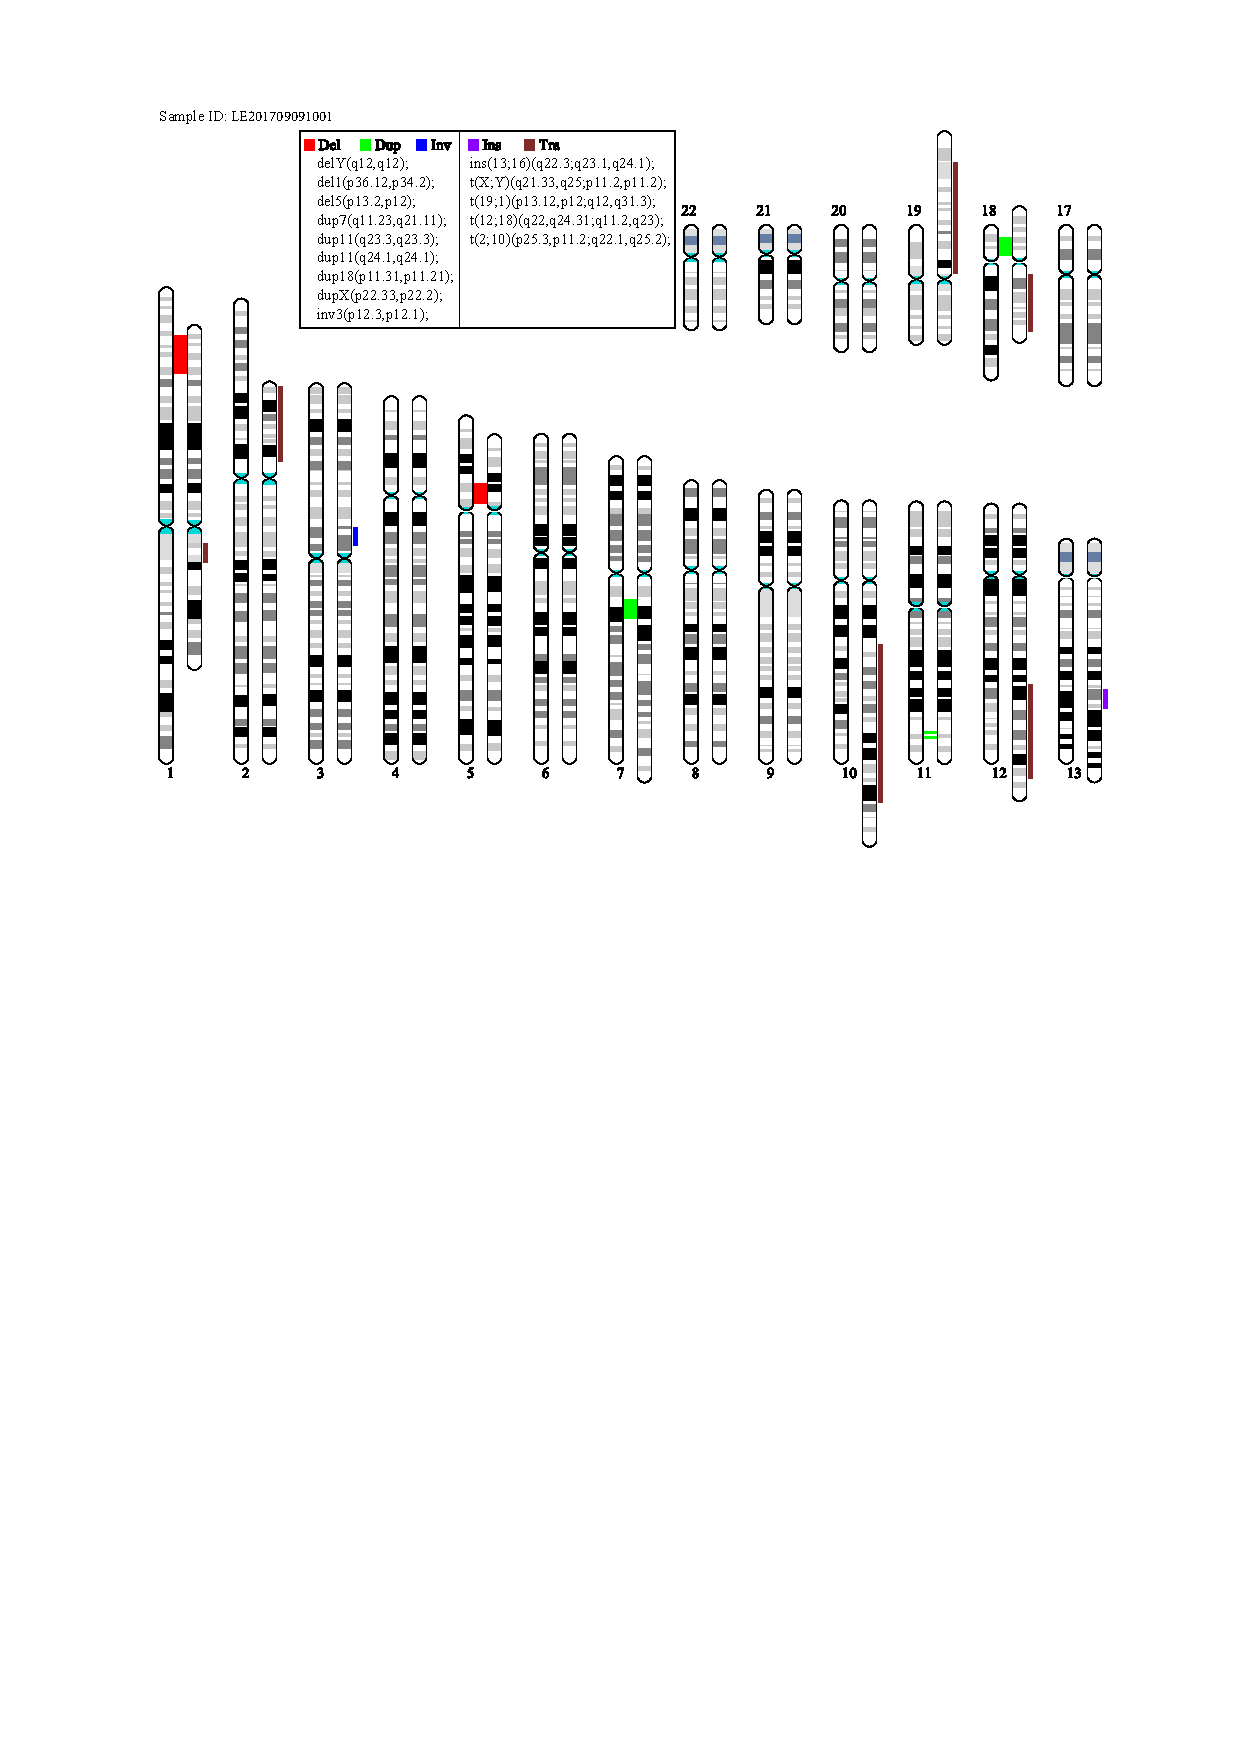
\includegraphics[width=\linewidth]{figures/electronical_idiogram.pdf}
	\end{figure}
	

\end{landscape}

\end{document}